\documentclass[letter,10pt,twoside]{article}

\usepackage[spanish,es-nodecimaldot]{babel}
\usepackage[utf8]{inputenc}

\renewcommand{\familydefault}{\sfdefault}
\usepackage[T1]{fontenc}
\usepackage{textcomp}

\usepackage{framed}
\usepackage[svgnames]{xcolor}
\colorlet{shadecolor}{Gainsboro!50}

\usepackage{enumitem}
\usepackage{graphicx}
\usepackage{pstricks}

\usepackage{anysize}
\marginsize{3cm}{2cm}{2cm}{3cm}

\usepackage{float}
\usepackage{siunitx}
\usepackage{amsmath}
\usepackage{array}

\usepackage{multicol}
\usepackage{pifont}

\usepackage{fancyhdr}
\usepackage{lastpage}
\pagestyle{fancy}
\fancyhf{}
\fancyhead[LE,RO]{Resistencia de los Materiales}
\fancyfoot[CO,CE]{\thepage\ de \pageref{LastPage}}

\special{papersize=215.9mm,279.4mm}

\usepackage[
    pdfauthor={Carlos Eduardo Caballero Burgoa},%
    pdftitle={Resistencia de los Materiales},%
    pdfsubject={Practica 02},%
    colorlinks,%
    citecolor=black,%
    filecolor=black,%
    linkcolor=black,%
    urlcolor=black,
    breaklinks]{hyperref}
\usepackage{breakurl}

\newcommand{\blankpage}{
\newpage
\thispagestyle{empty}
\mbox{}
\newpage
}

\renewcommand{\arraystretch}{1.2}

\begin{document}

\begin{titlepage}
\begin{center}
{\Large UNIVERSIDAD MAYOR DE SAN SIMÓN}\\
\vspace*{0.15cm}
{\large FACULTAD DE CIENCIAS Y TECNOLOGÍA}\\
\vspace*{9.0cm}
{\Large \textbf{PRACTICA No. 2}}\\
\end{center}

\vspace*{7.4cm}
\leftskip=7.95cm
\noindent
\textbf{Estudiante:}\\
Caballero Burgoa, Carlos Eduardo.\\
\textbf{Carrera:}\\
Ingeniería Electromecánica.\\
\newline
\textbf{Docente:}\\
Ing. Guido Gómez Ugarte.\\
\newline
\textbf{Fecha de entrega:} 30 de Septiembre del 2022.\\

\end{titlepage}

\blankpage

\colorbox{blue!25}{\textbf{PROBLEMA 1:}}

\begin{figure}[H]
\centering
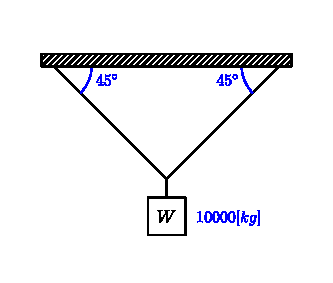
\includegraphics[scale=1.8]{resources/f01.eps}
\end{figure}

Hallar:
\begin{enumerate}
    \item Reacciones.
    \item {\O} del pasador P (SAE1010, $\sigma_f=2100[kg/cm^2]$, $n=2$).
        \begin{figure}[H]
        \centering
        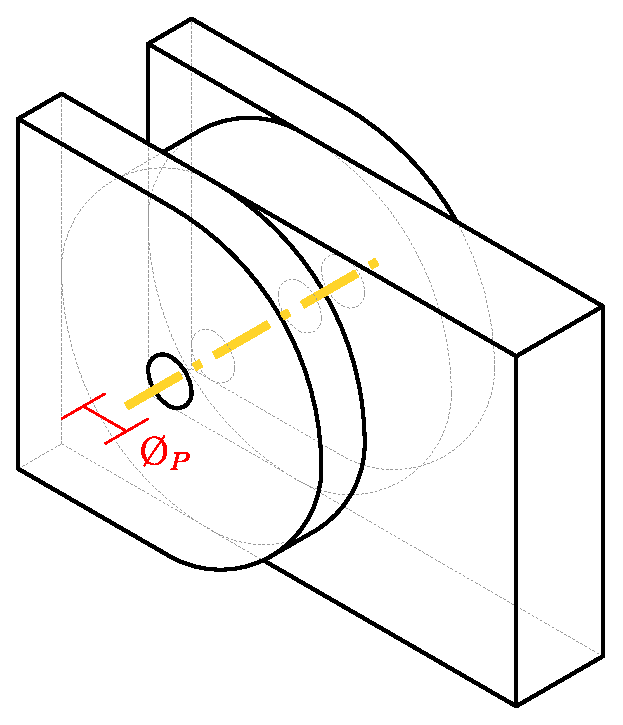
\includegraphics[scale=0.4]{resources/p01.eps}
        \end{figure}
    \item {\O} del cable Q (SAE1040, $\sigma_f=4200[kg/cm^2]$, $n=2$).
    \item {\O} de los pernos de anclaje (SAE1020, $\sigma_f=2500[kg/cm^2]$, $n=2$).
        \begin{figure}[H]
        \centering
        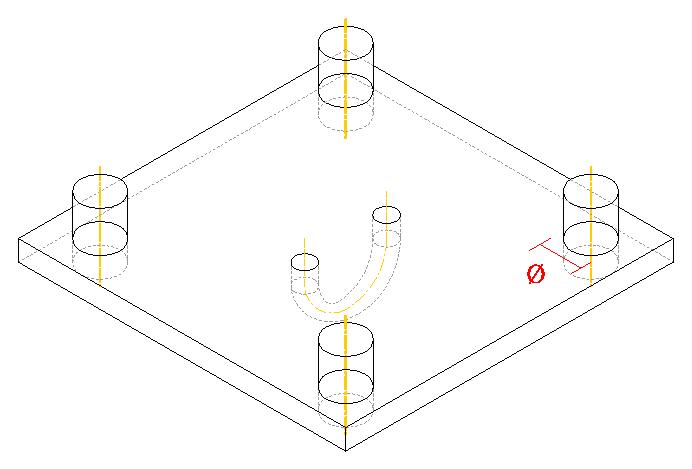
\includegraphics[scale=0.65]{resources/p02.eps}
        \end{figure}
\end{enumerate}

\textbf{\underline{Solución}:} \\

\textbf{Sistema no concurrente:} \\
Se plantean las ecuaciones de equilibrio:

\begin{equation*}
    \sum{F_x} = 0
\end{equation*}
\begin{equation*}
    \sum{F_y} = 0
\end{equation*}

Se consideran los siguientes puntos para el calculo de momentos:

\begin{figure}[H]
\centering
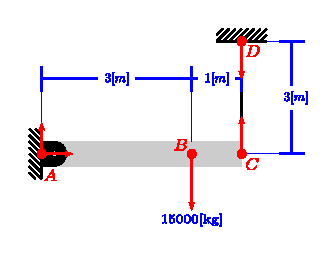
\includegraphics[scale=1.8]{resources/g01.eps}
\end{figure}

\begin{equation*}
    \sum{M_A} = 0
\end{equation*}
\begin{equation*}
    \sum{M_B} = 0
\end{equation*}
\begin{equation*}
    \sum{M_C} = 0
\end{equation*}

\textbf{Variables:} $A_x$, $A_y$, $C_y$.
\\

\begin{figure}[H]
\centering
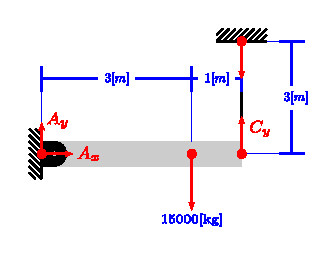
\includegraphics[scale=1.8]{resources/h01.eps}
\end{figure}

$\sum{F_x} = 0$:
\begin{equation*}
    A_x = 0
\end{equation*}

$\sum{F_y} = 0$:
\begin{equation*}
    A_y - 15000 + C_y = 0
\end{equation*}
\begin{equation*}
    A_y + C_y = 15000
\end{equation*}

$\sum{M_A} = 0$:
\begin{equation*}
    15000(3) - C_y(4) = 0
\end{equation*}
\begin{equation*}
    4 C_y = 45000
\end{equation*}
\begin{equation*}
    C_y = 11250
\end{equation*}

$\sum{M_B} = 0$:
\begin{equation*}
    A_y(3) - C_y(1) = 0
\end{equation*}
\begin{equation*}
    3 A_y - C_y = 0
\end{equation*}

$\sum{M_C} = 0$:
\begin{equation*}
    A_y(4) - 15000(1) = 0
\end{equation*}
\begin{equation*}
    4 A_y = 15000
\end{equation*}
\begin{equation*}
    A_y = 3750
\end{equation*}

\begin{equation*}
\boxed{
    \begin{array}{l}
        A_x = 0[\text{kg}] \\
        A_y = 3750[\text{kg}] \\
        C_y = 11250[\text{kg}]
    \end{array}
}
\end{equation*}

Por tanto:

\begin{equation*}
\boxed{
    \begin{array}{l}
        \text{Sistema isoestático}
    \end{array}
}
\end{equation*}

\textbf{{\O} del pasador P (Tensión cortante):}

\begin{equation*}
    \tau \le \bar{\tau}
\end{equation*}
\begin{equation*}
    \frac{F}{2A} \le \frac{0.5 \sigma_f}{n}
\end{equation*}
\begin{equation*}
    \frac{F}{2(\dfrac{\pi}{4} \text{\O}^2)} \le \frac{0.5 \sigma_f}{n}
\end{equation*}
\begin{equation*}
    \sqrt{\frac{n\,F(4)}{2\,\pi(0.5)\sigma_f}} \le \text{\O}
\end{equation*}
\begin{equation*}
    \sqrt{\frac{4\,n\,F}{\pi\sigma_f}} \le \text{\O}
\end{equation*}
\begin{equation*}
    \sqrt{\frac{4(2)(3750)}{\pi(2100)}} \le \text{\O}
\end{equation*}
\begin{equation*}
    2.1324[cm] \le \text{\O}
\end{equation*}

\begin{equation*}
\boxed{
    \begin{array}{l}
        \text{\O} \ge 21.324[mm] \\
        \text{\O} = \dfrac{7}{8}''
    \end{array}
}
\end{equation*}

\textbf{{\O} del cable Q (Tensión de tracción):}

\begin{equation*}
    \sigma \le \bar{\sigma}
\end{equation*}
\begin{equation*}
    \frac{F}{A} \le \frac{\sigma_f}{n}
\end{equation*}
\begin{equation*}
    \frac{F}{\dfrac{\pi}{4} \text{\O}^2} \le \frac{\sigma_f}{n}
\end{equation*}
\begin{equation*}
    \sqrt{\frac{n\,F(4)}{\pi\sigma_f}} \le \text{\O}
\end{equation*}
\begin{equation*}
    \sqrt{\frac{4\,n\,F}{\pi\sigma_f}} \le \text{\O}
\end{equation*}
\begin{equation*}
    \sqrt{\frac{4(2)(11250)}{\pi(4200)}} \le \text{\O}
\end{equation*}
\begin{equation*}
    2.6117[cm] \le \text{\O}
\end{equation*}

\begin{equation*}
\boxed{
    \begin{array}{l}
        \text{\O} \ge 26.117[mm] \\
        \text{\O} = 1\dfrac{1}{16}''
    \end{array}
}
\end{equation*}

\textbf{{\O} de los pernos de anclaje (Tensión de tracción):}

\begin{equation*}
    \tau \le \bar{\tau}
\end{equation*}
\begin{equation*}
    \frac{F}{4A} \le \frac{\sigma_f}{n}
\end{equation*}
\begin{equation*}
    \frac{F}{4(\dfrac{\pi}{4} \text{\O}^2)} \le \frac{\sigma_f}{n}
\end{equation*}
\begin{equation*}
    \sqrt{\frac{n\,F}{\pi\sigma_f}} \le \text{\O}
\end{equation*}
\begin{equation*}
    \sqrt{\frac{2(11250)}{\pi(2500)}} \le \text{\O}
\end{equation*}
\begin{equation*}
    1.6926[cm] \le \text{\O}
\end{equation*}

\begin{equation*}
\boxed{
    \begin{array}{l}
        \text{\O} \ge 16.926[mm] \\
        \text{\O} = \dfrac{11}{16}''
    \end{array}
}
\end{equation*}

\newpage

\colorbox{blue!25}{\textbf{PROBLEMA 2:}}

\begin{figure}[H]
\centering
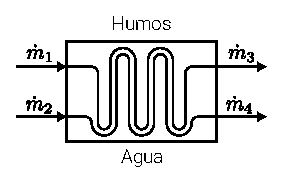
\includegraphics[scale=1.6]{resources/f02.eps}
\end{figure}

Hallar:
\begin{enumerate}
    \item $\text{\O}_1$, $\text{\O}_2$, $\text{\O}_3$ (SAE1020, $\sigma_f=2500[kg/cm^2]$, $n=2$).
\end{enumerate}

\textbf{\underline{Solución}:} \\

\textbf{$\text{\O}_1$ (Tensión de tracción):}

\begin{equation*}
    \sigma \le \bar{\sigma}
\end{equation*}
\begin{equation*}
    \frac{F}{A} \le \frac{\sigma_f}{n}
\end{equation*}
\begin{equation*}
    \frac{F}{\dfrac{\pi}{4} \text{\O}^2} \le \frac{\sigma_f}{n}
\end{equation*}
\begin{equation*}
    \sqrt{\frac{4\,n\,F}{\pi\sigma_f}} \le \text{\O}
\end{equation*}
\begin{equation*}
    \sqrt{\frac{4(2)(1000)}{\pi(2500)}} \le \text{\O}
\end{equation*}
\begin{equation*}
    1.0093[cm] \le \text{\O}
\end{equation*}

\begin{equation*}
\boxed{
    \begin{array}{l}
        \text{\O} \ge 10.093[mm] \\
        \text{\O} = \dfrac{13}{32}''
    \end{array}
}
\end{equation*}

\textbf{$\text{\O}_2$ (Tensión de compresión):}

\begin{equation*}
    \sigma \le \bar{\sigma}
\end{equation*}
\begin{equation*}
    \frac{F}{A} \le \frac{2\,\sigma_f}{n}
\end{equation*}
\begin{equation*}
    \frac{F}{\dfrac{\pi}{4} \text{\O}^2} \le \frac{2\,\sigma_f}{n}
\end{equation*}
\begin{equation*}
    \sqrt{\frac{4\,n\,F}{2\,\pi\sigma_f}} \le \text{\O}
\end{equation*}
\begin{equation*}
    \sqrt{\frac{4(2)(2000)}{2\,\pi(2500)}} \le \text{\O}
\end{equation*}
\begin{equation*}
    1.0093[cm] \le \text{\O}
\end{equation*}

\begin{equation*}
\boxed{
    \begin{array}{l}
        \text{\O} \ge 10.093[mm] \\
        \text{\O} = \dfrac{13}{32}''
    \end{array}
}
\end{equation*}

\textbf{$\text{\O}_3$ (Tensión de tracción):}

\begin{equation*}
    \sigma \le \bar{\sigma}
\end{equation*}
\begin{equation*}
    \frac{F}{A} \le \frac{\sigma_f}{n}
\end{equation*}
\begin{equation*}
    \frac{F}{\dfrac{\pi}{4} \text{\O}^2} \le \frac{\sigma_f}{n}
\end{equation*}
\begin{equation*}
    \sqrt{\frac{4\,n\,F}{\pi\sigma_f}} \le \text{\O}
\end{equation*}
\begin{equation*}
    \sqrt{\frac{4(2)(5000)}{\pi(2500)}} \le \text{\O}
\end{equation*}
\begin{equation*}
    2.2568[cm] \le \text{\O}
\end{equation*}

\begin{equation*}
\boxed{
    \begin{array}{l}
        \text{\O} \ge 22.568[mm] \\
        \text{\O} = \dfrac{15}{16}''
    \end{array}
}
\end{equation*}

\newpage

\colorbox{blue!25}{\textbf{PROBLEMA 3:}}

\begin{figure}[H]
\centering
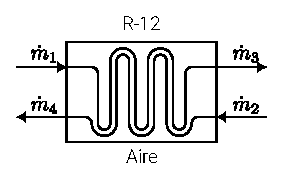
\includegraphics[scale=1.3]{resources/f03.eps}
\end{figure}

Hallar:
\begin{enumerate}
    \item $\text{\O}$ (SAE1010, $\sigma_f=2100[kg/cm^2]$, $n=2$).
\end{enumerate}

\textbf{\underline{Solución}:} \\

\begin{figure}[H]
\centering
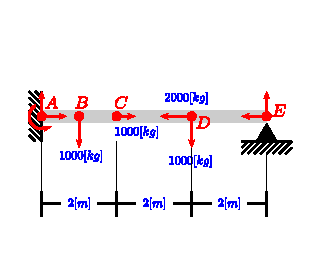
\includegraphics[scale=1.3]{resources/g03.eps}
\end{figure}

\begin{equation*}
    \tau \le \bar{\tau}
\end{equation*}
\begin{equation*}
    \frac{F}{4A} \le \frac{0.5 \sigma_f}{n}
\end{equation*}
\begin{equation*}
    \frac{F}{\dfrac{\pi}{4} \text{\O}^2} \le \frac{0.5 \sigma_f}{n}
\end{equation*}
\begin{equation*}
    \sqrt{\frac{4\,n\,F}{\pi(0.5)\sigma_f}} \le \text{\O}
\end{equation*}
\begin{equation*}
    \sqrt{\frac{4(2)(5000)}{\pi(0.5)(2100)}} \le \text{\O}
\end{equation*}
\begin{equation*}
    3.4823[cm] \le \text{\O}
\end{equation*}

\begin{equation*}
\boxed{
    \begin{array}{l}
        \text{\O} \ge 34.823[mm] \\
        \text{\O} = 1\dfrac{3}{8}''
    \end{array}
}
\end{equation*}

\colorbox{blue!25}{\textbf{PROBLEMA 4:}}

\begin{figure}[H]
\centering
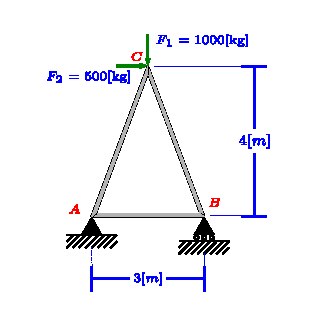
\includegraphics[scale=1.8]{resources/f04.eps}
\end{figure}

Hallar:
\begin{enumerate}
    \item Reacciones.
    \item {\O} del pasador A ($\sigma_f=4200[kg/cm^2]$, $n=2$).
    \item $\text{\O}_{AB}$, $\text{\O}_{BC}$, $\text{\O}_{CA}$ ($\sigma_f=2100[kg/cm^2]$, $n=2$).
\end{enumerate}

\textbf{\underline{Solución}:} \\

\textbf{Sistema no concurrente:} \\
Se plantean las ecuaciones de equilibrio:

\begin{equation*}
    \sum{F_x} = 0
\end{equation*}
\begin{equation*}
    \sum{F_y} = 0
\end{equation*}

Se consideran los siguientes puntos para el calculo de momentos:

\begin{figure}[H]
\centering
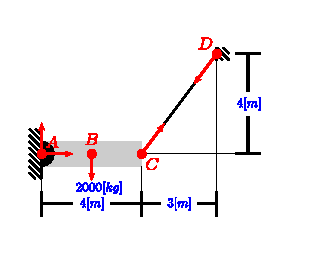
\includegraphics[scale=1.8]{resources/g04.eps}
\end{figure}

\begin{equation*}
    \sum{M_A} = 0
\end{equation*}
\begin{equation*}
    \sum{M_B} = 0
\end{equation*}
\begin{equation*}
    \sum{M_C} = 0
\end{equation*}

\textbf{Variables:} $A_x$, $A_y$, $B_y$.
\\

\begin{figure}[H]
\centering
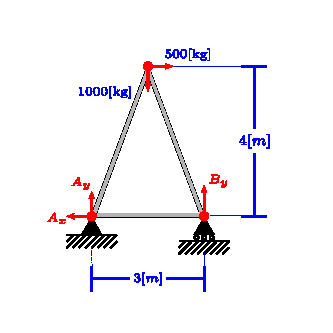
\includegraphics[scale=1.8]{resources/h04.eps}
\end{figure}

$\sum{F_x} = 0$:
\begin{equation*}
    A_x - 500 = 0
\end{equation*}
\begin{equation*}
    A_x = 500
\end{equation*}

$\sum{F_y} = 0$:
\begin{equation*}
    A_y + B_y - 1000 = 0
\end{equation*}
\begin{equation*}
    A_y + B_y = 1000
\end{equation*}

$\sum{M_A} = 0$:
\begin{equation*}
    500(4) + 1000(1.5) - B_y(3) = 0
\end{equation*}
\begin{equation*}
    3 B_y = 3500
\end{equation*}
\begin{equation*}
    B_y = 1166.7
\end{equation*}

$\sum{M_B} = 0$:
\begin{equation*}
    A_y (3) + 500 (4) - 1000(1.5) = 0
\end{equation*}
\begin{equation*}
    3 A_y = -500
\end{equation*}
\begin{equation*}
    A_y = -166.67
\end{equation*}

$\sum{M_C} = 0$:
\begin{equation*}
    A_x (4) + A_y (1.5) - B_y (1.5) = 0
\end{equation*}
\begin{equation*}
    4 A_x + 1.5 A_y - 1.5 B_y = 0
\end{equation*}

\begin{equation*}
\boxed{
    \begin{array}{l}
        A_x = 500[\text{kg}] \\
        A_y = -166.67[\text{kg}] \\
        B_y = 1166.7[\text{kg}]
    \end{array}
}
\end{equation*}

Por tanto:

\begin{equation*}
\boxed{
    \begin{array}{l}
        \text{Sistema isoestático}
    \end{array}
}
\end{equation*}

\textbf{{\O} del pasador A (Tensión cortante):}

\begin{equation*}
    \tau \le \bar{\tau}
\end{equation*}
\begin{equation*}
    \frac{F}{2A} \le \frac{0.5 \sigma_f}{n}
\end{equation*}
\begin{equation*}
    \frac{F}{2(\dfrac{\pi}{4} \text{\O}^2)} \le \frac{0.5 \sigma_f}{n}
\end{equation*}
\begin{equation*}
    \sqrt{\frac{n\,F(4)}{2\,\pi(0.5)\sigma_f}} \le \text{\O}
\end{equation*}
\begin{equation*}
    \sqrt{\frac{4\,n\,\sqrt{A_x^2 + A_y^2}}{\pi\sigma_f}} \le \text{\O}
\end{equation*}
\begin{equation*}
    \sqrt{\frac{4(2)\sqrt{500^2 + 166.67^2}}{\pi(4200)}} \le \text{\O}
\end{equation*}
\begin{equation*}
    0.5653[cm] \le \text{\O}
\end{equation*}

\begin{equation*}
\boxed{
    \begin{array}{l}
        \text{\O} \ge 5.653[mm] \\
        \text{\O} = \dfrac{15}{64}''
    \end{array}
}
\end{equation*}

\textbf{$\text{\O}_{AB}$, $\text{\O}_{BC}$, $\text{\O}_{CA}$:}

Se hallan las tensiones:

\begin{figure}[H]
\centering
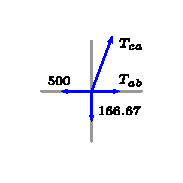
\includegraphics[scale=1.8]{resources/x0401.eps}
\end{figure}

\begin{equation*}
    \sum{F_x} = 0
\end{equation*}
\begin{equation*}
    T_{ab} + T_{ca}\,\left(\frac{1.5}{\sqrt{1.5^2+4^2}}\right) = 500
\end{equation*}

\begin{equation*}
    \sum{F_y} = 0
\end{equation*}
\begin{equation*}
    T_{ca}\,\left(\frac{4}{\sqrt{1.5^2+4^2}}\right) = 166.67
\end{equation*}

\begin{equation*}
    \begin{cases}
        T_{ca} = 178 \\
        T_{ab} = 437.5
    \end{cases}
\end{equation*}

\begin{figure}[H]
\centering
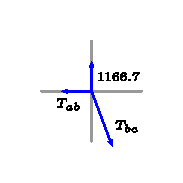
\includegraphics[scale=1.8]{resources/x0402.eps}
\end{figure}

\begin{equation*}
    \sum{F_x} = 0
\end{equation*}
\begin{equation*}
    T_{bc}\,\left(\frac{1.5}{\sqrt{1.5^2+4^2}}\right) - T_{ab} = 0
\end{equation*}

\begin{equation*}
    \sum{F_y} = 0
\end{equation*}
\begin{equation*}
    T_{bc}\,\left(\frac{4}{\sqrt{1.5^2+4^2}}\right) = 1167.7
\end{equation*}

\begin{equation*}
    \begin{cases}
        T_{bc} = 1246 \\
        T_{ab} = 437.50
    \end{cases}
\end{equation*}

\begin{figure}[H]
\centering
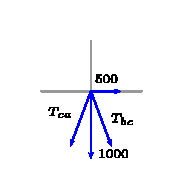
\includegraphics[scale=1.8]{resources/x0403.eps}
\end{figure}

\begin{equation*}
    \sum{F_x} = 0
\end{equation*}
\begin{equation*}
    500 + T_{bc}\,\left(\frac{1.5}{\sqrt{1.5^2+4^2}}\right) = T_{ca}\,\left(\frac{1.5}{\sqrt{1.5^2+4^2}}\right)
\end{equation*}

\begin{equation*}
    \sum{F_y} = 0
\end{equation*}
\begin{equation*}
    1000 + T_{ca}\,\left(\frac{4}{\sqrt{1.5^2+4^2}}\right) + T_{bc}\,\left(\frac{4}{\sqrt{1.5^2+4^2}}\right) = 0
\end{equation*}

\begin{equation*}
    \begin{cases}
        T_{bc} = -1246 \\
        T_{ca} = 178
    \end{cases}
\end{equation*}

Por tanto, las tensiones son:

\begin{figure}[H]
\centering
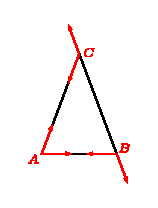
\includegraphics[scale=1.8]{resources/x0404.eps}
\end{figure}

\textbf{$\text{\O}_{ab}$ (Tensión de tracción):}

\begin{equation*}
    \sigma \le \bar{\sigma}
\end{equation*}
\begin{equation*}
    \frac{T_{ab}}{A} \le \frac{\sigma_f}{n}
\end{equation*}
\begin{equation*}
    \frac{T_{ab}}{\dfrac{\pi}{4} \text{\O}^2} \le \frac{\sigma_f}{n}
\end{equation*}
\begin{equation*}
    \sqrt{\frac{4\,n\,T_{ab}}{\pi\sigma_f}} \le \text{\O}
\end{equation*}
\begin{equation*}
    \sqrt{\frac{4(2)(437.5)}{\pi(2100)}} \le \text{\O}
\end{equation*}
\begin{equation*}
    0.7284[cm] \le \text{\O}
\end{equation*}

\begin{equation*}
\boxed{
    \begin{array}{l}
        \text{\O} \ge 7.284[mm] \\
        \text{\O} = \dfrac{5}{16}''
    \end{array}
}
\end{equation*}

\textbf{$\text{\O}_{bc}$ (Tensión de compresión):}

\begin{equation*}
    \sigma \le \bar{\sigma}
\end{equation*}
\begin{equation*}
    \frac{T_{bc}}{A} \le \frac{2\,\sigma_f}{n}
\end{equation*}
\begin{equation*}
    \frac{T_{bc}}{\dfrac{\pi}{4} \text{\O}^2} \le \frac{2\,\sigma_f}{n}
\end{equation*}
\begin{equation*}
    \sqrt{\frac{4\,n\,T_{bc}}{2\,\pi\sigma_f}} \le \text{\O}
\end{equation*}
\begin{equation*}
    \sqrt{\frac{4(2)(1246)}{2\,\pi(2100)}} \le \text{\O}
\end{equation*}
\begin{equation*}
    0.8692[cm] \le \text{\O}
\end{equation*}

\begin{equation*}
\boxed{
    \begin{array}{l}
        \text{\O} \ge 8.692[mm] \\
        \text{\O} = \dfrac{11}{32}''
    \end{array}
}
\end{equation*}

\textbf{$\text{\O}_{ca}$ (Tensión de tracción):}

\begin{equation*}
    \sigma \le \bar{\sigma}
\end{equation*}
\begin{equation*}
    \frac{T_{ca}}{A} \le \frac{\sigma_f}{n}
\end{equation*}
\begin{equation*}
    \frac{T_{ca}}{\dfrac{\pi}{4} \text{\O}^2} \le \frac{\sigma_f}{n}
\end{equation*}
\begin{equation*}
    \sqrt{\frac{4\,n\,T_{ca}}{\pi\sigma_f}} \le \text{\O}
\end{equation*}
\begin{equation*}
    \sqrt{\frac{4(2)(178)}{\pi(2100)}} \le \text{\O}
\end{equation*}
\begin{equation*}
    0.4646[cm] \le \text{\O}
\end{equation*}

\begin{equation*}
\boxed{
    \begin{array}{l}
        \text{\O} \ge 4.646[mm] \\
        \text{\O} = \dfrac{3}{16}''
    \end{array}
}
\end{equation*}

El diámetro es el máximo de los diámetros hallados:

\begin{equation*}
\boxed{
    \begin{array}{l}
        \text{\O}_{\text{max}} = max(\text{\O}_{ab},\text{\O}_{bc},\text{\O}_{ca}) = 8.692[mm] \\
        \text{\O}_{\text{max}} = \dfrac{11}{32}''
    \end{array}
}
\end{equation*}

\end{document}

